%==============================================================================
% Sjabloon poster bachproef
%==============================================================================
% Gebaseerd op document class `a0poster' door Gerlinde Kettl en Matthias Weiser
% Aangepast voor gebruik aan HOGENT door Jens Buysse en Bert Van Vreckem

\documentclass[a0,portrait]{hogent-poster}

% Info over de opleiding
\course{Bachelorproef}
\studyprogramme{toegepaste informatica}
\academicyear{2025-2026}
\institution{Hogeschool Gent, Valentin Vaerwyckweg 1, 9000 Gent}

% Info over de bachelorproef
\title{AI-ondersteunde taakverdeling voor IT-teams: een conceptueel model voor optimale taak-werknemer matching}
\author{Arthur Declercq}
\email{Arthur.declercq2@student.hogent.be}
\supervisor{Martine Van Audenrode}

% Indien ingevuld, wordt deze informatie toegevoegd aan het einde van de
% abstract. Zet in commentaar als je dit niet wilt.
\specialisation{AI \& Data Engineering}
\keywords{AI, taakallocatie, stress}
\projectrepo{https://github.com/ArthurDeclercq8/bachelorproef}

\begin{document}

\maketitle

\begin{abstract}
Stress komt in elke job voor. In deze bachelorproef wordt er gekeken naar de IT-sector. Waar gemiddeld 29\% van de Europese werknemers lijdt aan stress of depressie, loopt dat cijfer bij IT-professionals op tot bijna het dubbele. Een oorzaak hiervan is een onevenwichtige taakverdeling, dat geen rekening houdt met werkdruk of individuele capaciteiten. Dit onderzoek verkent hoe artificiële intelligentie de taakverdeling binnen IT-teams kan optimaliseren om werkdruk te verminderen en mentale gezondheid te ondersteunen. Via Python en scikit-learn werd een Random Forest-model getraind op synthetische data (22 werknemers, 300 taken) om voor elke werknemer-taakcombinatie een geschiktheidsscore te berekenen. Vergeleken met Round-Robin, Greedy Rol-Match en ChatGPT (GPT-4o) scoort het ML-model het tweede laagste op rol-match (71,7\%) en bereikt het ook de tweede meeste evenwichtige werklastdistributie (standaarddeviatie: 1,39 vs. 2,23–1,70 bij de alternatieven). Het is wel de enige methode die kwaliteit én werklastbalans systematisch combineert. Vervolgonderzoek kan zich richten op validatie in een reële bedrijfsomgeving, integratie van reinforcement learning en longitudinale meting van de impact op stressniveaus.
\end{abstract}

\begin{multicols}{2} % This is how many columns your poster will be broken into, a portrait poster is generally split into 2 columns

\section{Introductie}

Stress treft elke werknemer, maar in de IT-sector is het probleem bijzonder acuut. Waar op de Werelddag voor Geestelijke Gezondheid 2025 al 29\% van de Europese werknemers leed aan stress of depressie, verdubbelt dat cijfer wanneer enkel naar IT-professionals wordt gekeken. Een onderbelichte oorzaak hiervan is de manier waarop taken worden verdeeld: de huidige taakverdeling houdt te weinig rekening met de individuele capaciteiten, werkdruk en mentale belasting van werknemers. In dit onderzoek wordt onderzocht hoe een AI-gebaseerd model voor betere taakallocatie kan zorgen. Het eindresultaat is een goed onderbouwd AI-conceptmodel dat inzicht geeft in hoe een persoonlijk afgestemd takenpakket de werkdruk kan verminderen en daardoor de mentale gezondheid kan ondersteunen.
\section{Experimenten}

Het concept werd ontwikkeld in Python met scikit-learn, op basis van synthetisch gegenereerde data: 22 werknemers en 300 taken, waarvan 240 trainingstaken en 60 testtaken. Elke werknemer en taak werd voorzien van allerlei kenmerken zoals rol, werkdruk, persona-scores, taakcomplexiteit, etc. Via een heuristisch puntensysteem, dat gebaseerd is op rolmatch, persona-fit en werkdrukpenalty, werd een Random Forest classifier getraind met 200 beslissingsbomen. Het model voorspelt per werknemer-taakcombinatie een geschiktheidsscore, waarna de best scorende werknemer de taak ontvangt. Na elke toewijzing wordt de werkdruk dynamisch bijgewerkt, zodat het systeem taken op een meer realistische manier verdeelt.

\section{Sectie met figuur}

Om de meerwaarde van het ontwikkelde systeem te beoordelen, werd het vergeleken met drie andere allocatiemethodes: Round-Robin, Greedy Rol-Match en ChatGPT (GPT-4o). Alle methodes ontvingen exact dezelfde invoer: een testset van 60 taken en 22 werknemers. Ze werden beoordeeld aan de hand van zes kwantitatieve metrics: rol-match, werklastverdeling, gemiddelde eindwerkdruk, overbelasting, ervaringsfit en deadline-risico. De evaluatie werd volledig geautomatiseerd via een evaluatiescript, met uitzondering van ChatGPT, waarvoor de toewijzingen handmatig werden ingevoerd.

Hier staan de resultaten van het evaluatiescript.

\begin{center}
  \captionsetup{type=figure}
  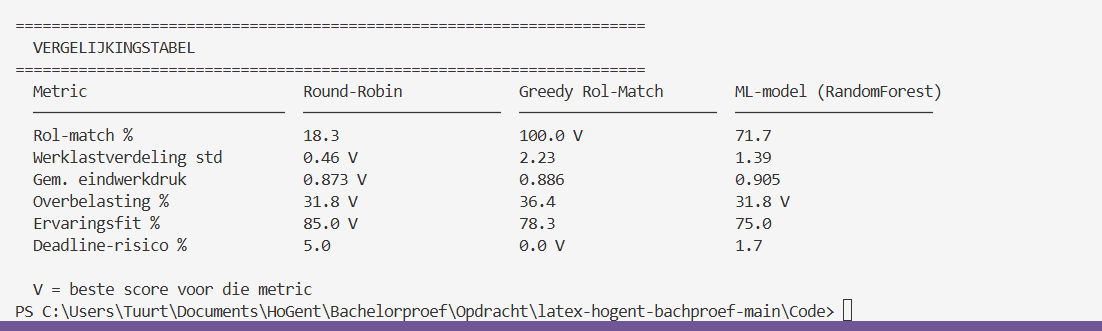
\includegraphics[width=1.0\linewidth]{../graphics/screenshot010.png}
  \captionof{Uitvoer evaluatiescript.py}{De uitvoer van het evaluatiescript.}
\end{center}

\section{Conclusies}

Het ontwikkelde ML-model is de enige geautomatiseerde methode die kwaliteit én werklastbalans systematisch combineert. Met een werklastverdeling van standaarddeviatie 1,39 presteert het duidelijker beter dan Greedy (2,23) en ChatGPT (1,70), terwijl de overbelasting (31,8\%) gelijk blijft aan Round-Robin. De lagere rol-match (71,7\% tegenover 100\% bij Greedy en ChatGPT) is geen tekortkoming, maar een bewuste afweging: het model verkiest soms een iets minder perfecte rol boven een overbelaste werknemer. Dit maakt het systeem duurzamer voor het welzijn van het team. De voornaamste beperking blijft de afhankelijkheid van synthetische trainingsdata. Voor productiegebruik is training op echte historische data noodzakelijk.

\section{Toekomstig onderzoek}

Verder onderzoek kan zich richten op verschillende pijlers: validatie in een reële bedrijfsomgeving met echte historische toewijzingsdata, de integratie van reinforcement learning zodat het systeem zichzelf continu verbetert op basis van praktijkfeedback en een longitudinale meting die nagaat of een evenwichtigere taakverdeling effectief leidt tot lagere stressniveaus bij IT-professionals.

\end{multicols}
\end{document}